\section{Prestudy}
\label{sec:prestudy}
%Intro - what the prestudy was
In order to inform the development of the project, and provide a reasonable basis for some of the design decisions made about the system, an initial prestudy was run with questions covering a wide range of relevant areas.
%Justifications - some detail about contents
The primary intention of the survey was to find out how people currently consume TV programmes and related streaming media, and their responses to the adverts that support the services they use.
There were questions on format and frequency of media consumption, and typical actions during advertisement presentation.
The study also included questions about individual levels of acceptance of the use of personal information for advertisement targeting, and an opportunity to share further personal opinions and comments in an optional free text question.
%Conclusion - the prestudy was useful
Ultimately, the wide coverage of questions gave many useful insights into existing viewer habits and responses.

%Intro - what the data was for
The main use of the data collected during the survey was to support and justify system development decisions throughout the course of the project. 
%Justification - specific hopes for the results
The questions were written to elicit information from the participants in support of several specific purposes, in addition to the basic background information about existing viewing habits.
One intended function of the results was to establish which features of an advert had the most influence on user attention -- this would allow development to be focused upon the best techniques to retain user attention to adverts, thereby making the product a more desirable option for advertisers, and resulting in greater profits for advertisers and greater satisfaction for users.
Another intended outcome was to discover whether typical advertisement responses provided scope for alternative attention retention techniques; for example, if users typically refocused their activities onto other devices during advertisement breaks, the provision of audio-only advertisements could provide an avenue for successful impressions despite loss of visual attention.
%Conclusion - the data was relevant
Determining how users respond to existing adverts in existing systems was an important prerequisite to tailoring development work so that the system is as effective as possible, and the survey questions were designed to support that aim.


% Purpose of the study:\\
% Collect data on how people consume media and adverts\\
% Inform the development of features for the project\\
% Elicit basic information about viewer habits

\subsection{Methodology}

%Intro - we wanted efficiency
To help ensure that the prestudy results were relevant and informative, close attention was paid to certain aspects of the study methodology.
%Justification - this was how we got it
%-Selected students as a sample - representative (find reference)\\
\citet{viacom} reports that young adults (the 18-24 demographic) watch TV on tablets more than any other demographic, and so the prestudy was directed largely towards this group. Additionally Project4's target audience is that of students, so to provide a more useful outcome for the client, this demographic was chosen. Finally the Project4 adverts, made available to us by Inqb8r, are all directed at the student audience and hence it would have been an unbalanced set if other demographics had been included in the studied set.
%-Protected results, ethics number 4315\\
Following the guidelines of the governing body, the questionnaire draft was submitted to ERGO, and received ethical approval to proceed (study number 4315). %TODO - mention password protected and automatic
%-Performed early\\
Since the survey outcomes were an important influencing factor in the continued development of the system, it was essential that the prestudy was completed early in the lifetime of the project. Once the intention and form of the questions had been finalised, the survey was created and publicised as swiftly as possible.
%Conclusion - aspects of how the survey was run made it more successful
By releasing the study quickly and advertising it specifically to the target demographic, maximal value was derived from the outcomes. %TODO: gah.

%Intro - we wanted lots of data
So that anomalous results did not unduly skew the outcome of the study, and to ensure broad coverage and increase the possible diversity of viewpoints captured, it was important to attempt to maximise the number of responses the survey would receive.
%Justification - we did these things to induce people to answer
%We were also keen to ensure that as many people as possible would provide useful information
%-Short and easy and anonymous\\
One approach taken was to make the questionnaire as quick and painless as possible to complete.
The survey design was intentionally short and minimal, with the majority of the questions answerable via checkboxes or radio-buttons.
In order to gauge the influence of certain factors, a Likert scale was used with 3-point items; these will have been familiar to respondents as they are a common survey technique \citep{trochim2007}.
No personally identifiable information was collected, and the only question requiring a full text answer was optional. %TODO: talk about using an URL %(who wrote this?)
%-Webpage\\
A web-based service was used to host the survey, which helped to ensure participant anonymity and data security, ease of access to the survey by participants, and also automatic answer collation and streamlined processing.
%-Spread via social networking sites\\
Finally, the survey itself was largely advertised via social networking sites. Aside from the benefits of serendipitous discovery, this also helped to ensure that potential participants were most likely to find the survey during times when they would also have opportunity to quickly complete it.
%Conclusion - This helped: we got a large number of results as discussed in the following section
Initially the prestudy completion target was set at 30 respondents, however due at least in part to the techniques employed in its design, the final count was more than double this figure. %TODO: is this too wooly?

%Note
The prestudy page as presented to participants is still available online\footnote{Your4 Prestudy Questionnaire -- \footurl{http://your4.tv/\#prestudy}}, and a listing of the questions can be found in Appendix~\ref{sec:appendix_prestudy_questions}. 


\subsection{Results}

%Stats
%Intro - the survey was in some respects more successful than hoped
In many respects the survey was more successful than anticipated.
%Justification
%-Over the course of a single week
Over the course of a single week, the online survey was seen and completed by a large number of participants.
%-67 student participants
In total, 67 responses were recorded, covering a wide variety of viewpoints and supplying several useful datapoints about viewer habits and responses.
%-Discovered specific features we should focus on
These led to a number of specific features that were selected for further attention - and a number that were disregarded.
%Conclusion - this was a good thing
In terms of depth and breadth of feedback received, the prestudy provided a sound, results-backed basis for many of the development decisions throughout the project.

%Specific outcomes
%INtro - there are some specific things we can pick up on
Some of the data recorded during the prestudy was particularly relevant to the system specification process, while other questions produced responses that were more useful for informing a fuller picture of the context and demographic background.
%Justification
%Bacground - section .1
For example, the first few questions were intended to give a clearer view of how often respondents watched streaming media in various formats, and how the attention paid to adverts varied by format -- revealing that most attention was given to adverts shown on live TV (see Section~\ref{sec:prestudy_media}).
%Relevant adverts - section .2
Other data revealed which specific aspects of an advert were likely to have an influence on whether it was watched by a viewer, as discussed in Section~\ref{sec:prestudy_influence}.
%Ability to skip adverts - section .3
When considering adverts that were not watched by viewers, it was also useful to discover what actions were typically taken instead (Section~\ref{sec:prestudy_alternatives}) in order to investigate alternative methods through which overall advert impressions could be reasonably maximised.
%Targeting
Additionally, the prestudy questions anticipated a likely direction for the project and investigated acceptance of the use of personal information to improve advertisement relevance, revealing that most of the respondents were comfortable with some degree of targeting.
%Conclusion - IN this light, suggests that the product we propose will improve the ...
The survey results suggest that the proposed product will most easily be able to improve upon existing offerings by providing a TV-like experience with specific additional functionality, rather than trying to pursue an experience more akin to that supplied by traditional in-browser video sources.

%Interesting free text responses
The optional free text section of the survey provided some additional insights into viewer perceptions of existing advertising.
%Intro - of particular note:
%Justification - find some of these
%Bought protein / was gay - overzealous
A few users complained of particular instances of advertisement targeting being intrusive and ``creepy'', or at the least over-zealous. 
Others stated that they actively boycotted certain products or services due to bad advertising.
Often there were specific annoyances listed, such as adverts that were deliberately placed to promote accidental interaction, or were obnoxiously noisy.
Three respondents talked about interacting with adverts -- all reported dislike of compulsory interaction, but viewed optional interaction as an enhancement.
A small number of viewers noted particularly good adverts, often from specific companies or websites. 
Finally, many responses mentioned a general desire for better adverts, with five respondents citing relevance as a positive factor.
%Conclusion - variety of viewpoints out there
A range of individual viewpoints are apparent from the data -- from viewers that avoid advertising of any kind, to those that are prepared to tolerate it to support free services, to the rare few that mention appreciating good adverts.


\subsubsection{Attention by media type}
\label{sec:prestudy_media}
%Question: How often do you pay attention to adverts served with the following media?
\begin{figure}[H]
	\centering
	\vspace{-10pt}
	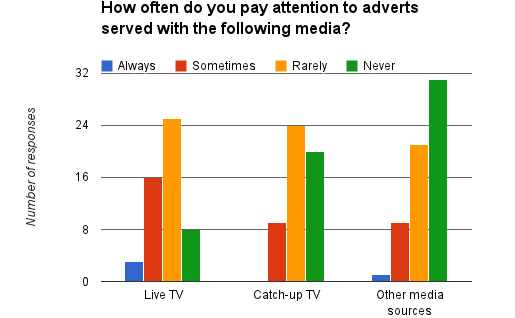
\includegraphics[width=0.7\textwidth, clip=true, trim=0 0 0 55pt]{images/prestudy_media.png}
	\caption{User responses to the question ``How often do you pay attention to adverts served with the following media?''}
	\label{fig:prestudy_media}
	\vspace{-15pt}
\end{figure}
As can be seen in Figure~\ref{fig:prestudy_media}, only a small minority of participants reported that they `Always' pay attention to adverts they are shown. In particular, amongst viewers watching other media such as Youtube, half of the respondents `Never' watch any advertisements at all -- in the free text responses, 12 of the respondents mentioned using ad-blocking programs. However, a far larger proportion of viewers `Always' or `Sometimes' watch adverts on live TV than on other formats, which indicates that a system similar to live TV may be most successful for advertisement delivery.

\subsubsection{Influential aspects}
\label{sec:prestudy_influence}
%Question: How much do the following aspects influence how likely you are to watch an advert?
\begin{figure}[H]
	\centering
	\vspace{-10pt}
	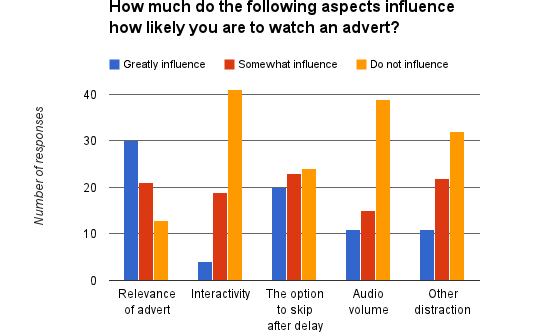
\includegraphics[width=0.7\textwidth, clip=true, trim=0 0 0 60pt]{images/prestudy_influence.png}
	\caption{User responses to the question ``How much do the following aspects influence how likely you are to watch an advert?''}
	\label{fig:prestudy_influence}
	\vspace{-25pt}
\end{figure}
The survey also looked at which specific aspects influenced whether viewers were likely to watch an advert, with results as shown in Figure~\ref{fig:prestudy_influence}. The factors with the largest influence were the relevance of the advertisement and whether or not there was opportunity to skip it -- these were selected as specific functionality to be further considered. 
The free text responses reveal that the question about interactivity is dominated by adverts that force a response from the user, whether they be obnoxiously loud, or require the user to interact with them before serving content. 
%TODO: do we mention the retrospecive need to define positive vs. negative influence?
One weakness seen in this question was that it only differentiates the magnitude of influence of a factor on viewers -- a 5-point Likert scale that added directionality (positive to negative influence) might have produced even more informative results.



\subsubsection{Advertisement responses}
\label{sec:prestudy_alternatives}
%Question: If you do not pay attention to adverts, which of the following do you do instead? (multiple choice)
\begin{figure}[H]
	\centering
	\vspace{-10pt}
	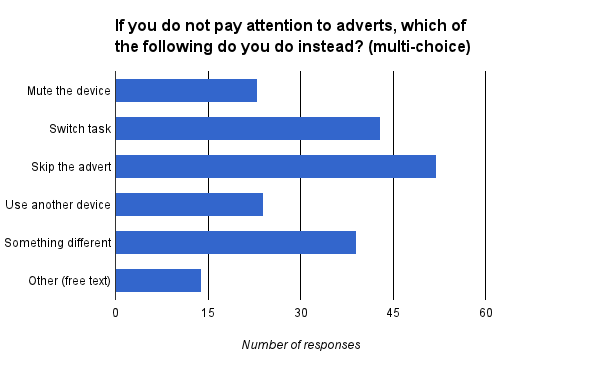
\includegraphics[width=0.7\textwidth, clip=true, trim=0 0 0 55pt]{images/prestudy_alternatives.png}
	\caption{User responses to the question ``If you do not pay attention to adverts, which of the following do you do instead?'' (multiple choice)}
	\label{fig:prestudy_alternatives}
	\vspace{-25pt}
\end{figure}
More than three quarters (52) of the respondents skip adverts at least occasionally if possible (Figure~\ref{fig:prestudy_alternatives}). Where respondents entered `Other' reasons, these were often references to ad-blocking programs or to `zoning out' and losing interest during advert breaks. Those who switched task did so to another task on the same device - presumably often to some form of channel listings.

